\documentclass[10pt,a4paper,titlepage]{article}
\usepackage{latexsym}
\usepackage[a4paper,top=2.5cm,bottom=2.5cm,left=2.5cm,right=2.5cm]{geometry}
\usepackage[utf8x]{inputenc}
\usepackage{booktabs,caption,amsfonts,amssymb,fancyhdr, amsmath}
\usepackage[english]{babel}
\usepackage{indentfirst}
\usepackage{multirow}
\usepackage{float}
\renewcommand*{\familydefault}{\sfdefault}
\usepackage{graphicx}
\usepackage{hyperref}
\usepackage{color}
\usepackage{subcaption}
\usepackage{listings}


\lstset{language=c++}
\lstset{backgroundcolor=\color{white}}
\lstset{frame=single}
\lstset{stringstyle=\ttfamily}
\lstset{keywordstyle=\color{red}\bfseries}
\lstset{commentstyle=\itshape\color{blue}}

\captionsetup[table]{position=top}
\addtolength{\textwidth}{1cm}
\addtolength{\hoffset}{-1cm}
\pagestyle{headings}



\begin{document}
\begin{center}
{\LARGE \bfseries Computational Physics\par}
\vspace{0.5cm}
{\LARGE \bfseries Project 3 \par}
\end{center}

\vspace{1cm}

\begin{tabular*}{\textwidth}{@{}l@{\extracolsep{\fill}}l@{}}
Academic year 2015-2016	 &Team group: \\
						&Giulio Isacchini\\
                        &Giovanni Pederiva\\
                        &Alessio Pizzini\\
                        &Mattia Ubertini\\
                                           
\end{tabular*}

\begin{center}
\hrule height 2 pt
\end{center} 

\section{Abstract}
The aim of this project is to compute numerically a six-dimensional integral, used to determine the ground state correlation energy between two electrons in a helium atom. This task has been achieved with different methods, namely: Gauss-Legendre quadrature, Gauss-Laguerre, brute force Monte Carlo and Monte Carlo with importance sampling. The results have then been compared and discussed. The code developed to solve the problem\footnote{The full code can be found on GitHub \url{https://github.com/GioPede/FYS3150/blob/master/Project3/main.cpp}} had also to be parallelized and a check of the time of computation was required.

\section{Analysis of the problem}
\subsection{Gaussian quadratures}

We approximate the wave function for two electrons in the helium atom with the product of the two single-particle hydrogen-like wave function:
\begin{equation}
\Psi({\bf r}_1,{\bf r}_2) = e^{-\alpha (r_1+r_2)}
\end{equation}
note that this wave function isn't normalized, but we will neglect that for our aim. 
We then want to compute the expectation value for the Coulomb interaction energy:
\begin{equation}\label{eq:correlationenergy}
   \langle \frac{1}{|{\bf r}_1-{\bf r}_2|} \rangle =
   \int_{-\infty}^{\infty} d{\bf r}_1d{\bf r}_2  e^{-2\alpha (r_1+r_2)}\frac{1}{|{\bf r}_1-{\bf r}_2|}.
\end{equation}
This integral can be solved analytically, resulting in $\frac{5\pi^{2}}{16^{2}}$. In the following analysis we will compare our results with this value.
At first we applied Gauss-Legendre quadrature to compute the integral. 
We will now use a set of orthonormal polynomials (e.g. Legendre, Laguerre...), defined on the interval $[a,b]$, where $a$, $b$ could also be $\pm \infty$. We now want to approximate our function with a polynomial of order $2N-1$, so
\begin{equation} 
\int_{a}^{b}f(x)dx \approx \int_{a}^{b}P_{2N-1}(x)dx = \sum_{i=1}^{N} w_i P_{2N-1}(x_i) \simeq \sum_{i=1}^{N} w_i f(x_i)=\sum_{i=1}^{N} \tilde{w}_i g(x_i)
\end{equation}
with $f(x)=W(x)g(x)$, $\tilde{w}_i =w_i W(x_i)$ and $x_i$ zeros of the orthogonal polynomials connected with the weight function $W(x)$.
\\Different integration intervals lead to different choices for the set of orthogonal polynomials and consequently to different weights $W(x_{k})$ and different functions $g(x)$.
\paragraph{Legendre polynomials} When the integration interval spans over a finite interval $[a,b]$ we use a particular set of orthogonal polynomials: Legendre Polynomials. 
\\Legendre  polynomials are defined over $[-1,1]$ and for these polynomials the weight functions are:
\begin{equation} 
W(x)= 1
\end{equation}
and the following orthogonality conditions holds for $m\neq n$:
\begin{equation}
\int_{-1}^{1}  L_{m}(x) L_{n}(x) dx=0
\end{equation}
and for $m=n$ the normality condition holds:
\begin{equation}
\int_{-1}^{1} \big(L_{n}(x)\big) ^2 dx=\frac{2}{2n+1}
\end{equation}
Finally Legendre polynomials can be defined in a recursive way: 
\begin{equation}
\textbf{L}_{0}(x)=1, \  
(j+1)\textbf{L}_{j+1}(x)+j\textbf{L}_{j-1}(x)-(2j+1)x\textbf{L}_{j}(x)=0.
\end{equation}
For evaluating the integral we approximate the function $f(x) \approx P_{2N-1}(x)$ and given the orthonormality of the Legendre Polynomials we can decompose the former polynomial as $$P_{2N-1}(x)=L_{N}(x)P_{N-1}(x)+Q_{N-1}(x)$$ 
Since the polynomial $P_{N-1}(x)$ can also be decomposed in terms of these orthonormal polynomials of degree $1$, $2$, ... $N-2$, $N-1$: 
\begin{equation}
P_{N-1}(x)=\sum_{k=0}^{N-1} \alpha_{k}L_{k}(x)
\end{equation}
we obtain:
\begin{equation}
\int_{a}^{b} P_{2N-1}(x)dx=\int_{a}^{b}(L_{N}(x)P_{N-1}(x)+Q_{N-1}(x))dx=\int_{a}^{b}Q_{N-1}(x)dx.
\end{equation}
Moreover, when $x$ equals one of the $N$ roots of $L_{N}$ we have $P_{2N-1}(x_{k})=Q_{N-1}(x_{k})$ exactly. We also note that evaluating our function $f(x)$ in these points, we obtain $N$ independent values which fully define the polynomial $Q_{N-1}$. Therefore, we will choose these points as mesh points.
Our aim now is to estimate our integral as 
\begin{equation}
\int_{a}^{b}f(x)dx \approx \int_{a}^{b}Q_{N-1}(x)dx \approx \sum_{k=1}^{N} \omega(x_{k})f(x_k)
\end{equation}
for some weights $w(x_k)$. In this case the integration interval is $[a,b]$, where $a,b$ $\in \mathbb{R}$ and it can be easily transformed into the interval $[-1,1]$ via a simple substitution $y=-1+\frac{2(x-a)}{b-a}$. It will be shown that such a choice leads to straight-forward calculations.

Turning back to equation (9), our following task is to develop $Q_{N-1}(x)$ in terms of Legendre polynomials: $Q_{N-1}(x) = \sum_{i=0}^{N-1}\alpha_{i}L_{i}$. Now, since $L_0(x)=1$ we get 
\begin{equation}
\int_{-1}^{1}Q_{N-1}(x)dx=\sum_{i=0}^{N-1}\alpha_{i}\int_{-1}^{1}L_{0}(x)L_{i}(x)dx=2\alpha_{0}
\end{equation}
due to orthonormality relations.
\\Defining the matrix $\textbf{L}$ as the matrix of the coefficients of Legendre polynomials and $\boldsymbol\alpha$ as the vector of the projection of the polynomial $\textbf{Q} _{N-1}$ along the $i$-th Legendre polynomial, the following relation holds:
\begin{equation}
\textbf{Q} _{N-1}(x_{k})=\textbf{L}\boldsymbol\alpha
\end{equation}
hence
\begin{equation}
\textbf{L} ^{-1}\textbf{Q} _{N-1}(x_{k})=\boldsymbol\alpha
\end{equation}
finally, exploiting both equation (11) and (13), we get:
\begin{equation}
\int_{-1}^{1}f(x)dx\approx \sum_{i=0}^{N-1}\omega_{i}f(x_{i})
\end{equation}
where $x_{i}$ are the zeros of the Legendre polynomial of degree $N$ and the vector of the weights is $$\tilde{w_i}=2(\textbf{L}^{-1})_{0i}$$. 
\paragraph{Laguerre polynomials} When the integration interval spans over an infinite interval, we need a different set of orthogonal polynomials. 
\\Laguerre polynomials are defined over $[0,\infty]$ and for these polynomials the weight functions are:
\begin{equation} 
W(x)= x^\alpha e^{-x}
\end{equation}
and the following orthogonality conditions holds for $m\neq n$:
\begin{equation}
\int_{0}^{\infty} x^\alpha e^{-x} G_{m}^\alpha(x)G_{n}^\alpha(x)dx=0
\end{equation}
and for $m=n$ the normality condition holds:
\begin{equation}
\int_{0}^{\infty} x^\alpha e^{-x} (G_{n}^\alpha(x))^2 dx=\frac{(n+\alpha)!}{n!}
\end{equation}

As before we want to find the weights $\tilde{w}_i$ of equation (3). Then
\begin{equation} 
\int_{0}^{\infty}f(x)dx = \int_{0}^{\infty}W(x)g(x)dx \approx\int_{0}^{\infty}W(x)P_{2N-1}(x)dx= \int_{0}^{\infty}W(x) \Big( G_{N}^\alpha(x)P_{N-1}(x)+Q_{N-1}(x) \Big) dx
\end{equation}
now the first factor of the former integral:
\begin{equation} 
\int_{0}^{\infty}W(x)G_{N}^\alpha(x)P_{N-1}(x)dx=\int_{0}^{\infty} x^\alpha e^{-x} G_{N}^\alpha(x)P_{N-1}(x)dx=0
\end{equation}
for the normalization condition of Laguerre polynomials. Now if we decompose Q with these polynomials: $Q_{N-1}(x)=\sum_{k=1}^{N-1}\beta_k G_k^\alpha(x)$
then we get
\begin{equation} 
\int_{0}^{\infty}f(x)dx \approx \int_{0}^{\infty}W(x)Q_{N-1}(x)dx=\sum_{k=1}^{N-1}\beta_k \int_{0}^{\infty} x^\alpha e^{-x}G_k^\alpha(x)G_0^\alpha(x)=\alpha! \beta_0 
\end{equation}
Defining the matrix $\textbf{G}$ as the matrix of the coefficients of Legendre polynomials and $\boldsymbol\beta$ as the vector of the projection of the polynomial $\textbf{Q} _{N-1}$ along the $i$-th Laguerre polynomial, the following relation holds:
\begin{equation}
\textbf{Q} _{N-1}(x_{k})=\textbf{G}\boldsymbol\beta
\end{equation}
hence
\begin{equation}
\textbf{G} ^{-1}\textbf{Q} _{N-1}(x_{k})=\boldsymbol\beta
\end{equation}
finally, exploiting both equation (20) and (22), we get:
\begin{equation}
\int_{0}^{\infty}f(x)dx\approx \sum_{i=0}^{N-1}\tilde{w}_if(x_{i})
\end{equation}
where $x_{i}$ are the zeros of the Laguerre polynomial of degree $N$ and the vector of the weights is \begin{equation}
\tilde{w}_i=\alpha!(\textbf{G}^{-1})_{0i}
\end{equation}
\newpage
\subsection{Monte Carlo method}
Then we turned to Monte Carlo method in order to get a smaller elapsed time. 
In its simplest form, i.e. when the integration interval is $[0,1]$ and a brute force Monte Carlo method is applied, it consists in computing
\begin{equation}
\langle f \rangle= \frac{1}{N} \sum_{i=1}^{N}f(x_{1})p(x_{i})
\end{equation}
where $p(x_{i})$ is the uniform distribution and the points $x_{i}$ are random generated via functions as \texttt{ran0}, \texttt{ran1}...
This method can be easily applied also to integrals which domain is in the form: $[a,b]$ via a change of variable.
Assuming that $f(x_{i})$ are independent, i.e. that our evaluating points $x_{i}$ are really randomly chosen, the variance reads:
\begin{equation}
\sigma^{2}_{N} \approx \frac{1}{N} (\langle f^{2} \rangle-\langle f \rangle^{2})= \frac{\sigma^{2}_{f}}{N}
\end{equation}
hence $\sigma_{N}\approx\frac{1}{\sqrt{N}}$.
On the other hand, traditional algorithms such as Gaussian quadrature have an error scaling as $\frac{1}{h^{k}}$, where $h$ is the steplength. or $N^{-\frac{k}{d}}$ since $N=(\frac{L}{h})^{d}$. It is now clear that Monte Carlo method is quicker for higher dimension integrals.
Monte Carlo method can be improved with a slightly different approach: instead of picking random points in the integration multidimensional interval, it would be better to collect more data where the value of the function is higher. To achieve that, let $p(y)$ be a PDF which profile resembles the function to be integrated (apart fron a scaling factor). Now,
\begin{equation}
I=\int_{a}^{b}f(y)dy=\int_{a}^{b}p(y)\frac{f(y)}{p(y)}dy
\end{equation}
And, performing a change of variable x $\rightarrow$ y:
\begin{equation}
x(y)=\int_{a}^{y}p(y')dy'
\end{equation}
we obtain 
\begin{equation}
I=\int_{0}^{1}\frac{f(y(x))}{p(y(x))}dx
\end{equation}
Now we can ran a plain Monte Carlo integration on the new function $\frac{f(y(x))}{p(y(x))}$, which is smoother than $f(x)$, e.g. its values are more similar each other, so now it is better to pick random points around the integration domain. Note that this is equivalent to say that we are picking more points where $p(y)$ has bigger values, i.e. where $f(y)$ does, since the two functions have about the same shape.
\newpage



\section{Data analysis}
\paragraph{Gaussian quadrature}First we have approched the problem exploiting the gaussian quadrature, using Legendre polynomials. In fact in cartesian coordinates we have an integral with simmetric integration points, as the domain of Legendre polynomials, which are defined in $[-1,1]$. The problem is that the integration domain goes from $-\infty$ to $+\infty$, the integral in cartesian coordinates reads:\begin{equation} \int_{-\infty}^{+\infty}\int_{-\infty}^{+\infty}\int_{-\infty}^{+\infty}\int_{-\infty}^{+\infty}\int_{-\infty}^{+\infty}\int_{-\infty}^{+\infty}e^{-4( \sqrt{x_2^2+y_2^2+z_2^2}+\sqrt{x_1^2+y_1^2+z_1^2})}\frac{dx_1dx_2dy_1dy_2dz_1dz_2}{\sqrt{(x_1-x_2)^2+(y_1-y_2)^2+(z_1-z_2)^2}}
\end{equation}
Obviously we cannot deal with infinity, but the function goes like $e^{-4(r_1+r_2)}$, this means that after a while the function is more or less zero everywhere, so the domain where the integral gets significant contributes is limited. Even if limiting the regions means to not take in count that there is an infinite line of singular points where the function diverges, but we have tested that these spikes outside the region does not contribute significantly to the values of integral, there is a representation in appendix, "fig.1", of simplified  version of the function in only two vaiables. 
Actually we have also put a statement in our code to avoid points with the denominator smaller than $10^{-10}$ inside the region, because if we did not do that we would have evaluated the function in this points and consequently the sum would have blown up.
\\
In this case we have tested many combinations of number of integration points and the extension of the domain and we have found that we get the best results with the domain defined between $[-3,3]$ with 25 integration points. So using the function \texttt{gauleg} defined in the library \texttt{lib.h} we have computed the weight function and we have estimated the integral as $I=  \sum_{k=1}^N w_k[x_k] f[x_k]$ 
getting $I=0.19581657$ against the real value   $0.192765711$ so we can see that the result is right just at the second leading digit. Adding more points actually doesn't seem to improve the result, as with the same domain with $30$ points we get $I=0.17728296$ that it's farther than then the previous one. As we can see this method is not so satisfactory, it's very unstable fixed the domain the value of integral can vary a lot changing the number of integration points in an unpredictable way. Moreover it requires a lot of calculations in particularly 6 nested loop, which means that we have to do, with $N$ the number of integration points, $N^6$ iterations and each iteration involves around 40 operations, for these reasons we can't deal with many integration points. 
\\
So we can say that this method is not suitable for many dimensional integrals.
\paragraph{Laguerre}The next attempt has been made again with the Gaussian quadrature but this time we have used a mix of Legendre and Laguerre polynomials. We have started writing the integral in spherical coordinates and the integral reads: \begin{equation} I=\int_{0}^{+\infty}\int_{0}^{+\infty}\int_{0}^{2 \pi}\int_{0}^{2 \pi}\int_{0}^{\pi}\int_{0}^{\pi} e^{-4(r_1+r_2)}\frac{r_1^2dr_1r_2^2dr_2sin(\theta_1)d\theta_1sin(\theta_2)d\theta_2d\phi_1d\phi_2}{\sqrt{r_1^2+r_2^2-2r_1r_2cos\alpha}}
\end{equation}
with $cos(\alpha)=cos(\theta_1)cos(\theta_2)+sin(\theta_1)sin(\theta_2)cos(\phi_1-\phi_2)$. Being the Laguerre polynomial defined in the interval $[0,+\infty]$ we have tried to use them for the variables $r_1$ and $r_2$ and we have kept the Legendre polynomials for the angles. 
\\
The best result got is with $N=15$ and it's $I_{15}=0.19328534$ again is right until the second leading digit. Actually the result of the integral computed in this way seems to converge to a value higher than this, as adding more points we get values $I_{20}=0.19478558$ $I_{25}=0.19480424$ $I_{30}=0.19477877$.
\\
But this method seems to be more stable than the previous one as we can see in the range for $20<N<30$ the value of the integral varies at the fourth leading digit, remaining in a 1\% margin from the real value. So even if this method is not so precise at least it seems to be more trustable, but for sure is giving more reasonable values already with 10 points. To sum up and compare the different results of the two algorithm we show a table of the computed values:
\begin{center}
\begin{tabular}{|c|c|c|}
\hline
Number of integration points          &  $I_{Leg}$    &  $I_{LL}$               \\\hline
$10$ &  $0.07197968$ & $0.17708077$ \\ \hline
$15$ & $0.23908829$ & $0.19328534$ \\\hline
$20$ & $0.15613939$ & $0.19478558$  \\\hline
$25$ & $0.19581657$ & $0.19480424$  \\\hline
$30$ & $0.17728296$ & $ 0.19477877$ \\\hline
\end{tabular}

\end{center}

We have noticed that the values of the integral got with the second method is always overestimated. 
It is strange since we have cut off some points, where the denominator is very small, so the value of the function would be very high, for this reason we were expecting that the computed values were smaller than the exact one. This means that it's not the most relevant source of error in this case.

\paragraph{Monte Carlo} For the last method to be used we ran four different types of integrations. The first one was a very basic algorithm which used the uniform distribution to get random points over a fixed interval; we chose the limits in the same way as we did for the Gaussian-Legendre quadrature, namely $(-3,3)$. The next integral was transformed from carthesian coordinates to spherical ones, however we still set an interval for the radial coordinate, form 0 to 4.\\ 
For the third one we used spherical coordinates and we also made a change of variables for the radial coordinate to make it cover all the range from 0 to infinity. We used the mapping $y(x)=-ln(1-x)$, where x is a number generated by a RNG with uniform distribution. We also had to multiply the integrand function with the proper jacobian.\\
Lastly we computed the integral using spherical coordinates, still with the variable change,  and importance sampling. We used the function $ p(x) = e^{-4x}$ as the new probability function which simplified a lot our integrand function as well. In this way we made the function smoother and  it has been possible to sample it mainly where its values were bigger, instead of collecting a lot of points in regions where it is basically 0.
In figure 3, in appendix, we have plotted a model in two variables of the function after the importance sampling.\\
In the next two tables we report the results we got from the different integrations with their respective standard deviation.\\
\begin{center}
\begin{tabular}{|c|c|c|c|c|}
\hline
Number of           &  Brute        & \multirow{2}{*}{$\sigma_{BF}$}&   Brute Force            &\multirow{2}{*}{$\sigma_{BFP}$} \\
Integration Points  &  Force        &                               &   Spherical Coordinates  &                                \\\hline
$10^5$              &  0.15954391   &   0.03455319                  &   0.18810667             &   0.00303888                   \\\hline
$10^6$              &  0.17754983   &   0.01529653                  &   0.19083326             &   0.00102753                   \\\hline
$10^7$              &  0.20796502   &   0.01066741                  &   0.19295919             &   0.00032727                   \\\hline
$10^8$              &  0.19370220   &   0.00289679                  &   0.19286204             &   0.00010375                   \\\hline
\end{tabular}
\captionof{table}{{\footnotesize  Limited integration interval results with different numbers of mesh points. The exact value of the integral to compare them with is $0.192765711$}}
\end{center}

\begin{center}
\begin{tabular}{|c|c|c|c|c|}
\hline
Number of           &  Spherical    & \multirow{2}{*}{$\sigma_{SC}$}&   Spherical Coordinates with  &\multirow{2}{*}{$\sigma_{IS}$}  \\
Integration Points  &  Coordinates  &                               &   Importance Sampling         &                                \\\hline
$10^5$              &  0.19205151   &   0.00298317                  &   0.19329349                  & 0.00295920                     \\\hline
$10^6$              &  0.19296413   &   0.00101211                  &   0.19294079                  & 0.00101166                     \\\hline
$10^7$              &  0.19306043   &   0.00032235                  &   0.19273239                  & 0.00032384                     \\\hline
$10^8$              &  0.19275195   &   0.00010444                  &   0.19284794                  & 0.00010382                     \\\hline
\end{tabular}
\captionof{table}{{\footnotesize  Unlimited integration interval results with different numbers of mesh points. The exact value of the integral to compare them with is $0.192765711$}}
\end{center}
As we can see the standard deviation keeps lowering as we increase the number of integration points, as expected. However the most interesting information is obtained by looking at the convergence of the different methods. The brute force integral requires a lot of points for its value to get close to the analytical one and remains the integral with the highest $\sigma$. The integral with the spherical coordinates with no variable change gives much better results with already $10^6$ integration points, and with one million points has already just an error of around 10\% in respect to the analytical solution and with $10^7$ it's almost exact.\\
The change of variables is what improves significantly the integral: with just a hundred thousand points the discrepancy between the numerical result and the exact solution is less than 1\%, which is really impressive. Increasing integration points anyways does still improve the results. The last integral, the one with important sampling, is almost exact for all the choices of number of integration points we made, however increasing this parameter leads to significantly lower $\sigma$, so this is still something we might want to do. The importance sampling allows to compute the integral with really few points much less then the Gaussian quadrature and the brute force Monte Carlo. 

\paragraph{Time Analysis and Parallelization} One of the goals of this project was to implement in our code some parallelized loops. We used the OpenMP library which is used for shared memories architectures, like the laptops we ran our code on. The changes to the code are really trivial, but the speed-up is really considerable. In the table we present all the algorithms we used and the execution time of each of them for the maximum number of points we tested them with. The machine that was used had 8 cores to run the program on.\\
\begin{center}
\begin{tabular}{|c|c|c|c|}
\hline
\multirow{2}{*}{Method} & Number of       			& Single    & 8 Processes  \\
                        &Iterations       			& Process   & in Parallel  \\\hline
Gauss-Legendre          &$\approx 250 \cdot 10^6$	& 17.340 s  & 04.812 s     \\\hline
Gauss-Laguerre          &$\approx 250 \cdot 10^6$	& 58.298 s  & 16.495 s     \\\hline
Brute-force MC          &  $10^8$   	  			& 16.393 s  & 04.035 s     \\\hline
BF spherical MC         &  $10^8$         			& 37.610 s  & 09.112 s     \\\hline
MC with variable change &  $10^8$         			& 47.528 s  & 11.365 s     \\\hline
MC with importance sampling & $10^8$      			& 44.911 s  & 10.523 s     \\\hline
\end{tabular}
\captionof{table}{{\footnotesize  Times of computation for the different integrals. Note that the gaussian quadratures were evaluated with more than twice as much points.}}
\end{center}
As we can see running times are all decreased after the parallelization, not exactly by a factor 0.125, but very close to a factor 0.25. This could be due to the fact that we set up the parallel calculation in a way that avoids data races, this means that some processors at times have to wait for the others to finish their operations, loosing a bit of time. By running again the code on just four cores we got a factor 0.3 in respect to the non parallelized time. This seems to confirm (it's not a real proof, it's just a guess) that the time of execution is not linearly correlated with the number of cores, but there is an asymptotic limit given by the operation on shared variables stored in memory.\\
This time analysis however showed us also that the less stable Gauss-Legendre and the Brute-Force Monte Carlo method are by far the fastest. Especially the latter even if it is very unstable in its results can still be considered a fair method, because it requires some really basic implementation and it can be run with much more integration points than all the others in the same time and as we have seen before the results with many points are quite good anyway and they seem to converge. The huge difference in time between the Brute Force integral and the other Monte Carlo integrals we have computed is mainly given by the higher complexity of the function to evaluate. The function in spherical coordinates contains sines and cosine functions, which require more time to compute than basic operations.\\

\section{Conclusions}
Gaussian quadrature with Legendre polynomials resulted to be the least reliable method, since it depends strongly on the number of integration points. Laguerre polynomials provided with much more precise results but resulted to be about four times more time consuming than the previous algorithm. 
\\ Monte Carlo method provided with much more precise results. The plain brute force algorithm with limited integration intervals resulted in being way less time consuming than the other ones, but gave results with about the same reliability as the ones provided by Gaussian quadrature. On the other hand, a simple change of coordinates in the brute force method resulted in more precise results than Gaussian quadrature with Laguerre polynomials with a smaller elapsed time. Finally, a change of coordinates and the implementation of importance sampling increased the precision of our results.
As for our estimation of the $\sigma$ of our results, it is strongly underrated for limited integral intervals, while it matches with our results for unlimited ones. 
\newpage
\section{Appendix}
\begin{figure}[H]
	\begin{center}
        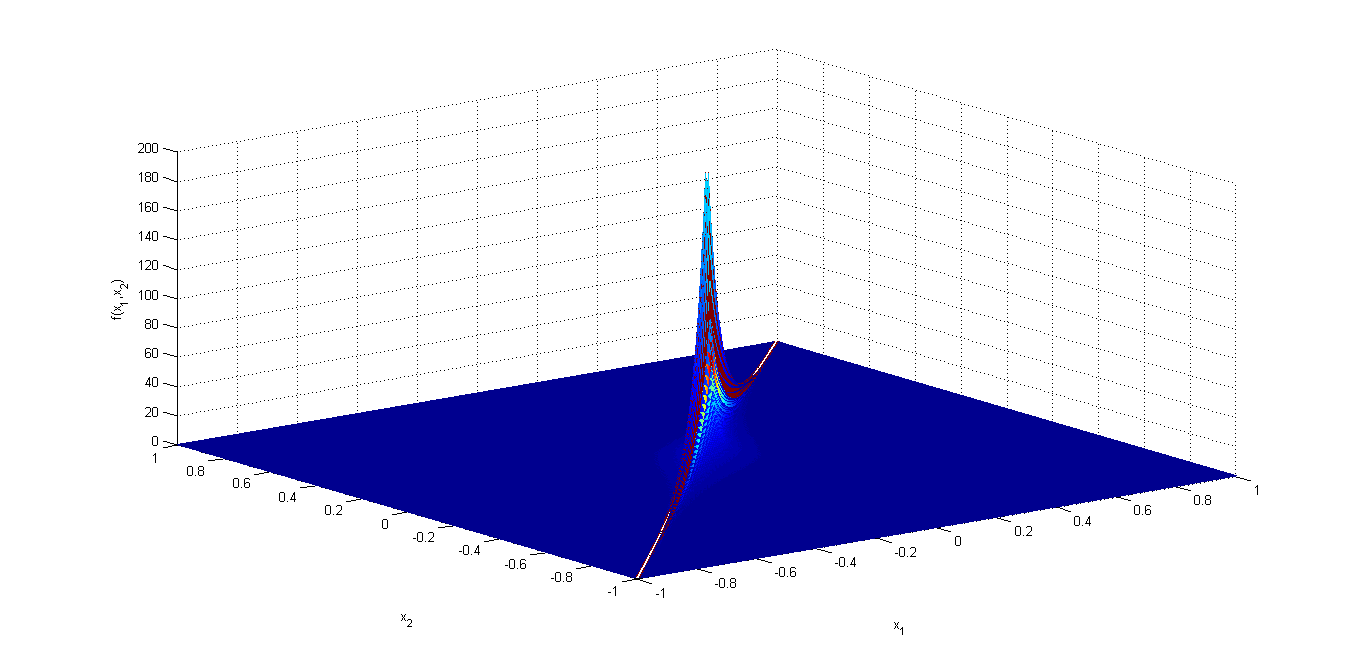
\includegraphics[width=0.69\textwidth]{f.png}
    	\caption{A simplified two dimensional version of the function we are integrating. The graph looks to be cut because the points next to the singularity aren't plotted}
	\end{center}
\end{figure}
\begin{figure}[H]
	\begin{center}
        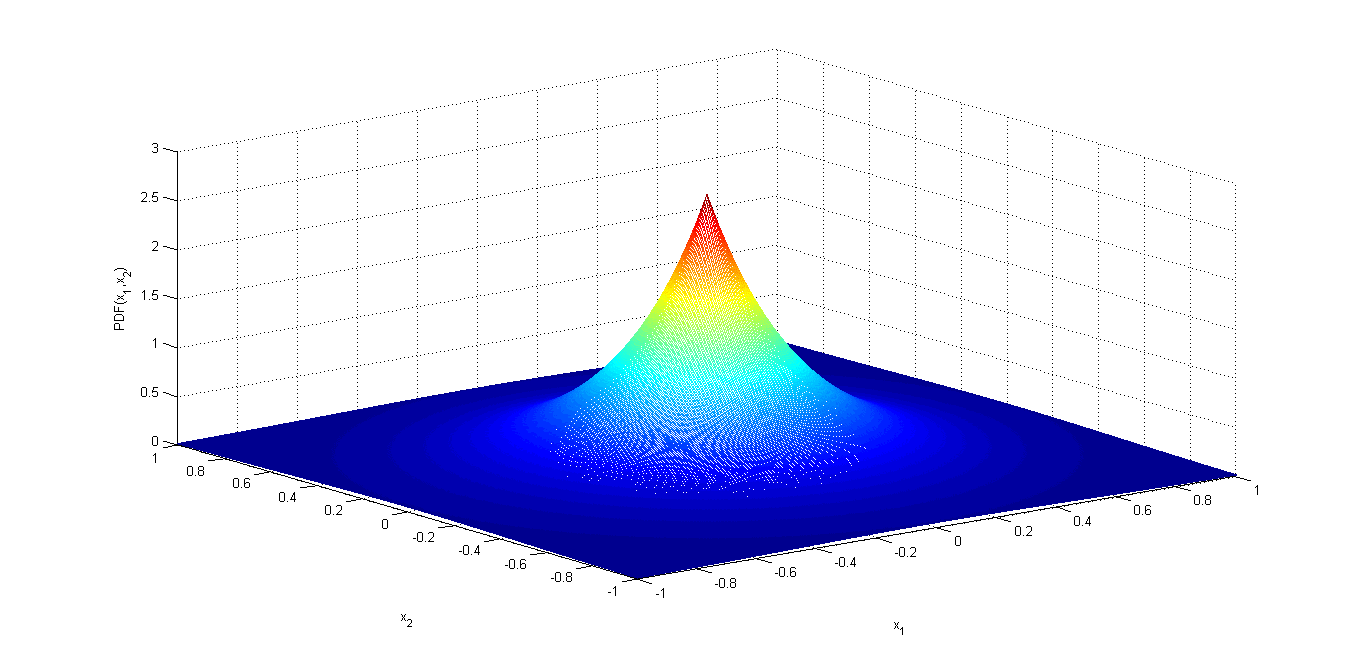
\includegraphics[width=0.69\textwidth]{correction.png}
    	\caption{A simplified version of the PDF function. Comparing it with the previous graph, it is clear that this choice allows us to pick more integration points where $f(x_1,x_2)$ has bigger values}
	\end{center}
\end{figure}
\begin{figure}[H]
\begin{center}
    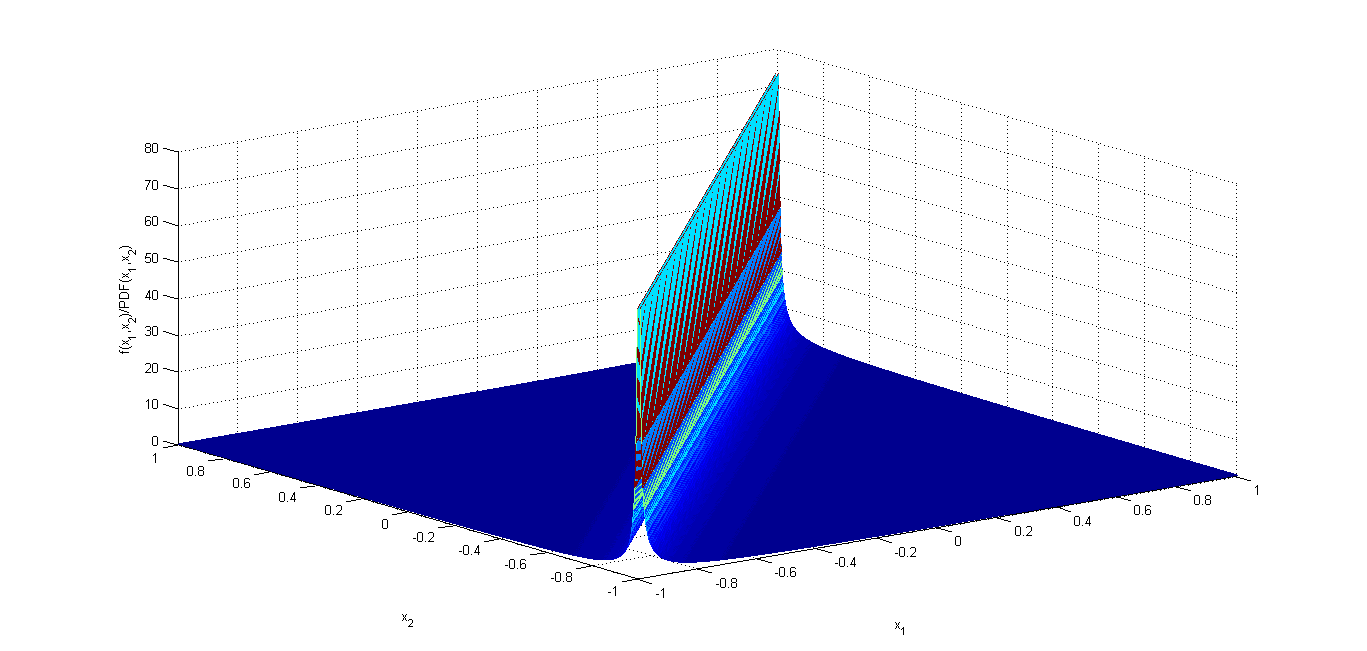
\includegraphics[width=0.69\textwidth]{result.png}
\caption{A simplified version of the original function $f(x_1,x_2)$ divided by $PDF(x_1,x_2)$. The function doesn't look flatter than the original one because the PDF we have chosen doesn't cancel the singularity. Despite this, we can see that now our function is significantly different from zero for a larger number of points than before}
	\end{center}
\end{figure}
\end{document}